\chapter{Migration process} \label{cha:migration}

This chapter describes the process of migrating a web application to serverless architecture. The goal of the process is to explore the catalogued patterns' feasibility by applying them on common problems in the domain of web application development. As well as exploring the patterns we're seeing how the distinct serverless features drive application design and trying to gain deeper understanding of the advantages and shortcomings of the paradigm. The chapter begins with the description of the migrated application along with its functional and non-functional requirements. We then identify the ways in which the current implementation fails to meet these requirements and thus set a target for the serverless implementation. Lastly a new serverless design is proposed using the pattern catalogue of chapter \ref{cha:patterns}, and in cases where the patterns prove insufficient or unsuitable to the problem in hand, modifications or new patterns are proposed.

\section{Image Manager}

The migrated application, Image Manager, is a tool for managing image assets. Image Manager is adapted from a real-world application, although modified in places for the sake of illustration. Similarly to a SaaS offering such as Cloudinary, the application takes user-uploaded images, performs various forms of processing and then hosts and serves the processed images to be consumed by other applications. In case of Image Manager the processing needs are threefold: rendering a thumbnail, rendering a low quality image placeholder (LQIP), and automatic label detection. Thus in short Image Manager can be split into three basic functional requirements: image upload, image processing and image hosting.

The pre-migration (or \textit{serverful}) Image Manager consists of a single server application that connects to a number of BaaS-type cloud services. These components are depicted in figure \ref{fig:serverfulArchitecture}. The server application publishes an HTTP API endpoint for image uploads which is consumed by a browser client. In place of access control this public-facing API uses a CAPTCHA: before image upload the client requests a challenge from Google reCAPTCHA API, solves it and sends the obtained token along with the image upload request. The server application then also connects to reCAPTCHA API to verify token validity before proceeding with the upload request. A CAPTCHA is used instead of full-blown authentication to allow for anonymous users while still providing some degree of protection against bots and other illicit usage. After CAPTCHA verification the application proceeds with image processing. The thumbnail and LQIP rendering tasks are performed locally whereas labeling is handled by a network call to an external image analysis service, Google Cloud Vision API. The three processing tasks are independent and performed concurrently. Finally both the original and processed images are uploaded to Google Cloud Storage where they can be fetched via publicly accessible URLs. This image upload sequence is illustrated in further detail in figure \ref{fig:serverfulSequence}.

\begin{figure}[H]
  \centering
  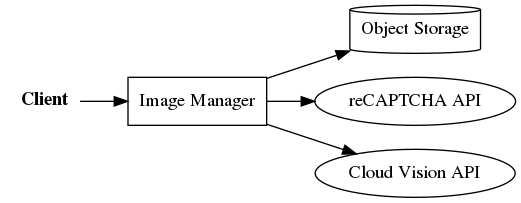
\includegraphics[width=0.65\textwidth]{image-manager.png}
  \caption{Image Manager components}
  \label{fig:serverfulArchitecture}
\end{figure}

\begin{figure}[H]
  \centering
  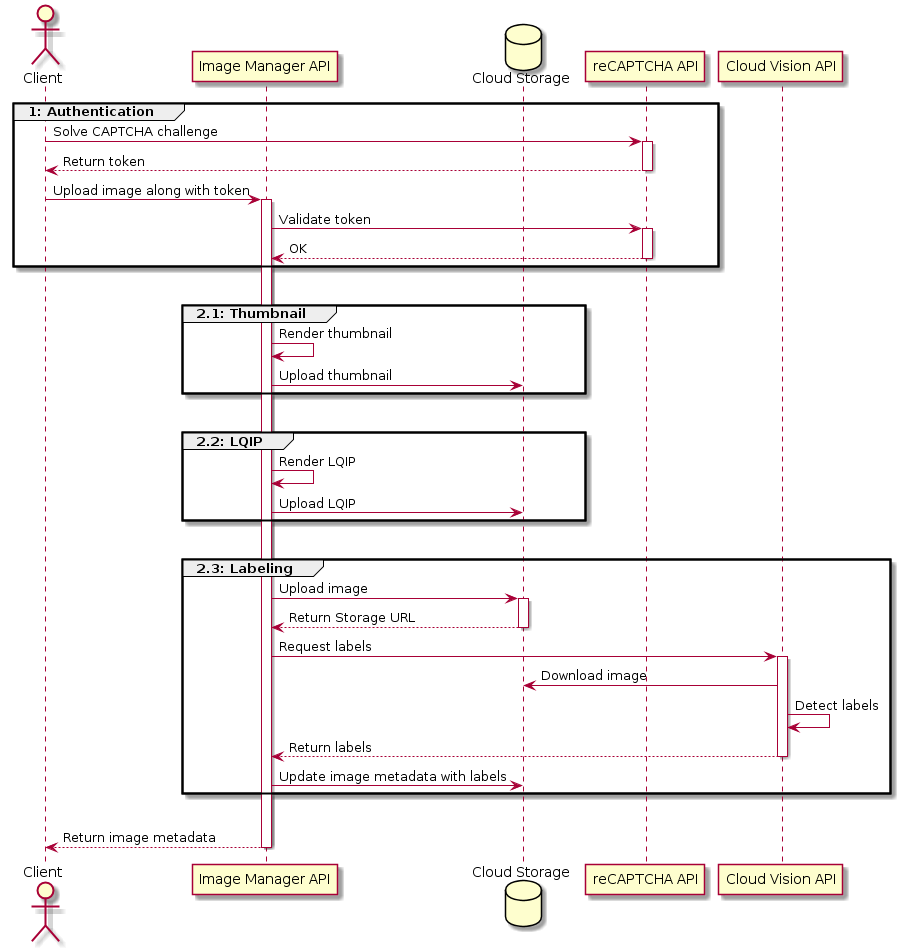
\includegraphics[width=1\textwidth]{sequence.png}
  \caption{Image Manager upload sequence}
  \label{fig:serverfulSequence}
\end{figure}

Overall the image upload task is both CPU-intensive due to rendering and I/O-heavy due to service requests and also since processing results are temporarily written on disk before cloud storage upload. As for technical details, Image Manager is written in TypeScript, transpiled into JavaScript and running on NodeJS v10. The server application is containerized into a Docker image and deployed on a single VM on Google Cloud Platform's us-east1 region. The VM exposes an IP address through which the application is accessed from public internet.

Image Manager can even in its pre-migration state be considered ``cloud-ready'' in the sense that it was originally designed and developed to run specifically in a cloud environment \parencite{pozdniakova17cloudready}. This is reflected in the usage of container technology and the reliance on cloud platform services in favour of self-managed code. The degree of cloud-readiness should be kept in mind when considering the migration process as the practices and observations might not apply when starting off with a more conventional on-premise application architecture.

The motivation to migrate Image Manager to serverless architecture stems from a number of shortcomings in the current implementation, specifically relating to the non-functional requirements of availability, scalability, cost-efficiency and isolation. First, the obvious drawback of the server application's single-VM deployment is poor availability as there is no failover instance to take over in case of VM failure. Likewise the application's capacity to serve traffic is limited by a single VM's computing resources as there is no scaling mechanism in play. Achieving this double goal of availability and scalability, i.e. ensuring a correct number of VMs to meet current demand at all times would require a considerable amount of infrastructure configuration involving load balancing, clusterization and scaling policies \parencite{jonas19berkeleyView}. This inelasticity also results in cost-inefficiency as the VM instance is constantly running and accumulating charges whether or not there's any traffic. Lack of isolation is also a major concern, primarily since all application logic including image processing tasks are bundled together into a single monolithic application. This causes resource contention, as for example high CPU usage in one of the rendering tasks can divert resources from the API and result in connection timeouts. This combined with processing tasks' highly asymmetrical performance profiles also further complicates scaling as we can only scale the whole application, not just the bottlenecks. Lack of isolation also presents itself in how all traffic is routed through the server application, which in case of image uploads means an extra network trip before reaching Cloud Storage. Finally, the server application's monolithic design has negative maintainability implications since modifications cannot be developed or deployed independently.

\section{Serverless Image Manager}

Rewriting an application in serverless architecture is clearly not a trivial task nor does it have a single correct solution. Comparable to building a system out of microservices or plotting class hierarchy in object-oriented software design, the same outcome can be achieved with a variety of different but equally valid compositions of FaaS and BaaS components. As a baseline the serverless Image Manager should fulfill the same functional requirements as its predecessor. Building on that the migration should improve the application's quality attributes, particularly concerning the deficiencies listed above.

Looking at Image Manager's components in figure \ref{fig:serverfulArchitecture}, it's notable that the system's non-functional deficiencies stem from the server application and not from the integrated cloud services. The services are fully provider-managed, scale to demand and follow a pay-per-use pricing model: they don't constitute an operational overhead nor limit the application's elasticity scaling- or pricing-wise. A serverless Image Manager can therefore retain these integrations while reimplementing the server application in FaaS. While the services themselves remain the same, what changes is the way they're interfaced with since a FaaS consumer can necessitate different communication patterns than a conventional one: publish-subscribe instead of request-response, for example. As for the server application, it has two main responsibilities: first, it acts as a glue component that binds together BaaS components. Second, it provides the kind of custom server-side functionality that we cannot or choose not to offload to external services, namely thumbnail and LQIP rendering. Seeing how these responsibilities match identically with the role of FaaS in serverless systems as discussed in section \ref{sec:faasbaas}, we can expect FaaS to provide a fitting serverless alternative and migration target for the server application. The specific FaaS platform used here is Cloud Functions \parencite{google18cloudFunctions} due to all the integrated services and the previous VM deployment residing on Google Cloud as well.

The simplest FaaS implementation of Image Manager involves wrapping the whole server application into a single function that is then invoked synchronously via HTTP. This arrangement is from the client's point of view identical to the container deployment since the function's exposed HTTP trigger acts just like the server application's HTTP API. It also already manages to shift a majority of operational concerns on to the cloud provider. However in many cases this approach is limited by the platform's restrictions on function size and computing resources. A single monolithic function also does little to improve isolation and maintainability. If allowed by platform limits the approach can nonetheless be a good starting point for migration: akin to the Strangler pattern (\ref{subsec:strangler}) first migrate the application into a single function and then incrementally split it off into smaller units.

\subsection{Pattern selection}

Taking full advantage of the FaaS platform's capabilities requires a more thorough redesign than simply packaging an application as-is into a single function. The design process used here is based on the pattern catalogue of chapter \ref{cha:patterns}. First each pattern is evaluated against the migrated application's functional and non-functional requirements. The patterns that most closely work towards meeting these requirements are then selected, and the selected patterns are finally composed together to form the proposed serverless design. Applying the process to Image Manager resulted in the following set of patterns: Event Processor, Fan-out/Fan-in, Thick Client, Valet Key and Bulkhead.

First of all the requirement for cost-efficiency leads towards the Event Processor pattern (\ref{subsec:Eventprocessing}). The image processing tasks should be event-driven: executed on-demand whenever there are images to process and not consume any resources or amass charges otherwise. Technically this is implemented by splitting image processing into a new function that subscribes to Cloud Storage upload events so that each image upload triggers a function invocation. The pattern also improves scalability since a large number of uploads results in a similarly large number of function invocations.

The requirement for scalability leads towards the Fan-out/Fan-in pattern (\ref{subsec:FanoutFanin}). In our case the pattern consists of splitting the three image processing tasks into their own functions: a simple decision to make with the tasks already being essentially independent. As each upload now triggers not one but three parallel functions, CPU-intensive rendering tasks can scale independently from the less intensive labeling task. Moreover We can expect a performance benefit as the overall task is completed faster.

The Thick Client pattern (\ref{subsec:thickClient}) is selected with cost-efficiency in mind. Since the Event Processor breaks coupling between the API and image processing, it is now possible to omit the API layer and have the client orchestrate uploads instead. Retaining the API would mean paying for function execution for the duration of image upload; by uploading images from the client directly to Cloud Storage this expense as well as an extra network trip can be avoided.

The Valet Key pattern (\ref{subsec:valetKey}) is chosen to authorize requests between the client and Cloud Storage and thus facilitate the client-driven workflow. This involves extending the CAPTCHA validation behaviour so that a temporary access token to Cloud Storage is returned in case of a valid CAPTCHA. Applying the Bulkhead pattern (\ref{subsec:Bulkhead}), the Valet Key implementation is split off into a separate authorizer function to ensure its availability when the rest of the system is under high load. The Function Warmer pattern (\ref{subsec:FunctionWarmer}) could optionally be used to further improve the authorizer's availability by keeping a warm function instance ready to serve requests at all times. In case of Image Manager there are no strict response time requirements so this pattern is omitted.

The design process results in the proposed design of the serverless Image Manager. This outcome is presented in figure \ref{fig:serverlessArchitecture} where rectangular blocks with a $\lambda$ prefix signify a FaaS function. In the serverless Image Manager the server application is replaced by four different functions: one for each image processing task plus an authorizer function. Out of these functions only the authorizer exposes an HTTP API whereas the others are event-driven. The new image upload sequence, as illustrated in figure \ref{fig:serverlessSequence}, is also more event-driven as opposed to being orchestrated by the server application.

\begin{figure}[H]
  \centering
  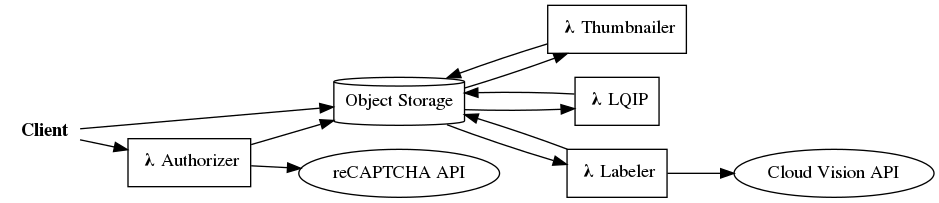
\includegraphics[width=\textwidth]{image-manager-serverless.png}
  \caption{Serverless Image Manager components}
  \label{fig:serverlessArchitecture}
\end{figure}

\begin{figure}[H]
  \centering
  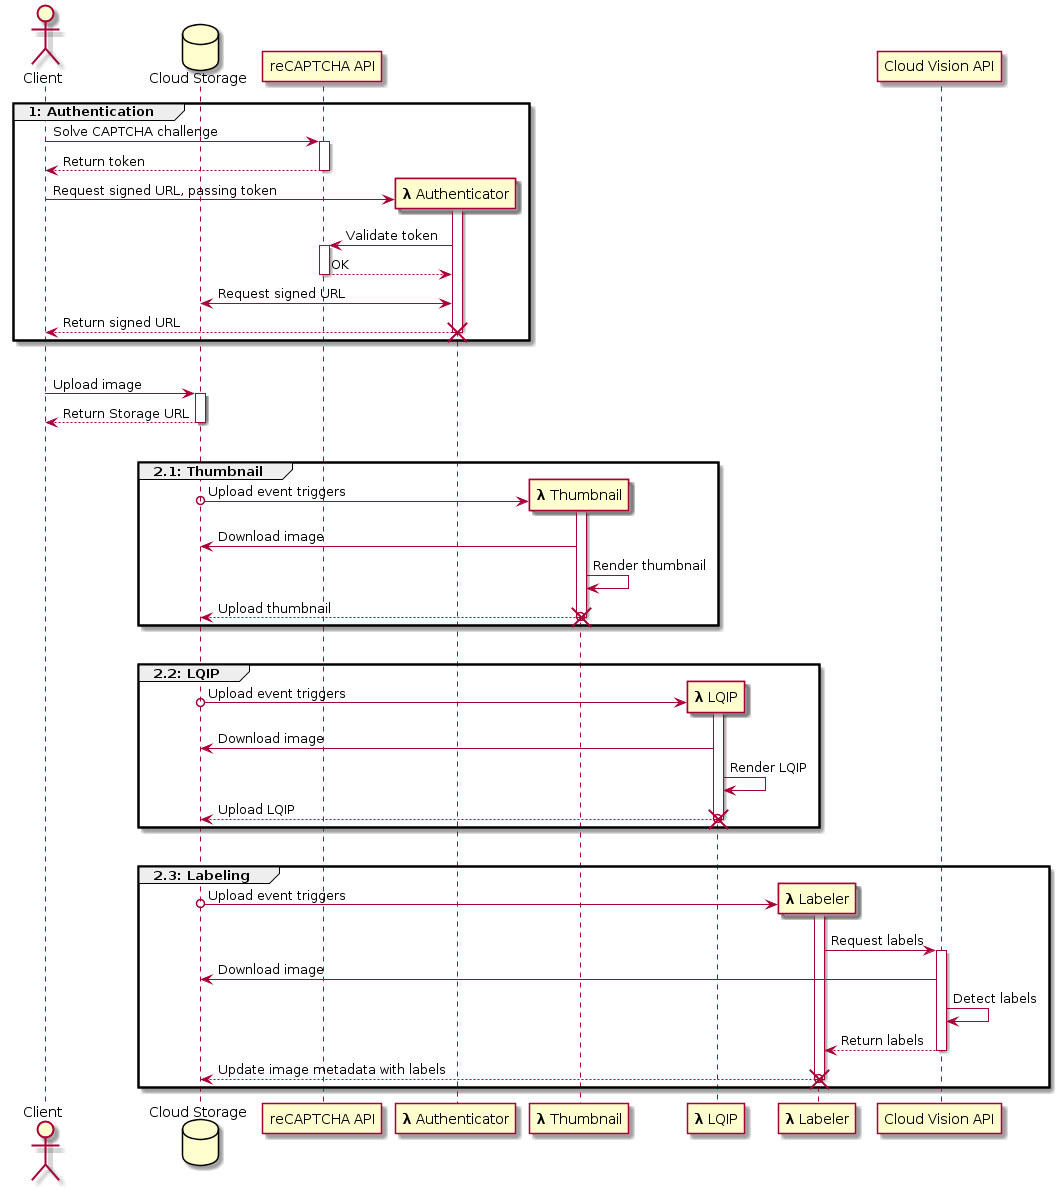
\includegraphics[width=1\textwidth]{sequence-serverless.png}
  \caption{Serverless Image Manager upload sequence (steps 2.1-2.3 run in parallel)}
  \label{fig:serverlessSequence}
\end{figure}

\section{New patterns} \label{sec:newPatterns}

This section lists five new patterns extracted from migration process. The patterns present solutions to problems in Image Manager's serverless design e.g. in places where the serverless implementation performs worse than the original one or fails to provide the same behaviour. In addition we're introducing patterns that could be used to extend the serverless design to further improve its quality or add functionality beyond the original requirements.

\subsection{Async Response} \label{subsec:AsyncResponse}

\textbf{Problem:} Client doesn't get any feedback from the asynchronous tasks it triggers.

\begin{figure}[h]
  \centering
  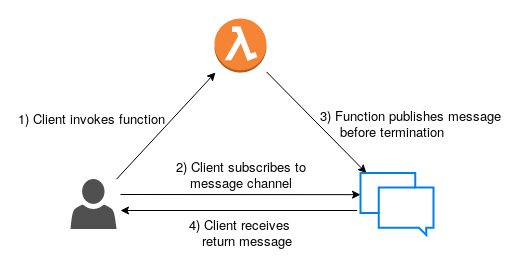
\includegraphics[width=0.7\textwidth]{patterns/async-response.png}
  \caption{Async Response}
  \label{fig:asyncResponse}
\end{figure}

\textbf{Solution:} Use a pub/sub channel to notify the client before function termination.

In the pre-migration Image Manager all processing happens in the span of the single upload request. The request blocks and the client won't receive a response before all processing and storage uploads are finished. On the other hand the serverless Image Manager client only receives an acknowledgment of receipt of the original image since image processing is continued asynchronously after the initial Cloud Storage upload. This means the serverless client has no way of notifying the user of a finished processing task. Solving this problem requires a way for the image processing functions to notify the client after they finished with execution.

In more general terms the problem is one of an asynchronously invoked function instance re-establishing communication with the original task initiator, i.e. turning fire-and-forget into something more resembling of request-and-response semantics. As additional complexity, the initiator might not be the actual function invoker but further down the call stack, as in the case of Image Manager where client first activates Cloud Storage which then invokes processing functions.

The Async Response pattern tackles the problem using publish-subscribe messaging. The client, after initiating the task, subscribes to a message channel and waits for notification of the task completion. Conversely the last function responsible for task execution publishes a message to the same channel before terminating. After receiving acknowledgment of task completion the client can dismantle the message channel and proceed to update the the user interface, for example. Instead of a single completion message we could also send status messages during execution for the client to keep track of task progress.

The Async Response can be implemented with any technology that enables publish-subscribe messaging between the client and function: Firebase Realtime Database on Google Cloud or API Gateway Websockets on AWS, for example. One implementation challenge concerns identifying the completion message: how should the message be sent so that it ends up at the right client? One approach is to wrap task initialization in another function that first creates a message channel with an unique identifier and then passes the identifier to both the client and the processing function. This however incurs the overhead of having to pass the channel identifier along each processing step. Another approach is to compute the channel identifier from task payload: in case of Image Manager the client could for example listen to messages on a channel named after the uploaded file's name.

\subsection{Task Controller} \label{subsec:taskManager}

\textbf{Problem:} Client has no way of controlling or cancelling an asynchronous task after triggering it.

\begin{figure}[h]
  \centering
  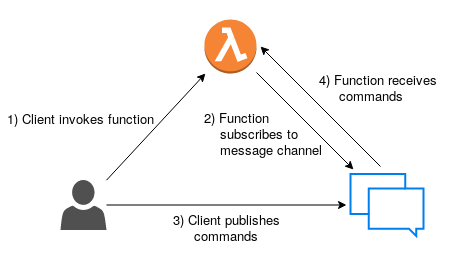
\includegraphics[width=0.65\textwidth]{patterns/task-controller.png}
  \caption{Task Controller}
  \label{fig:taskController}
\end{figure}

\textbf{Solution:} Make each function instance open a messaging channel to the client in the beginning of its execution in order to listen to client commands.

Possible future use cases for Image Manager would be to track processing task progress and cancel processing tasks midway. We could for example want to terminate a long-running and expensive batch job if its made redundant before completion, or tweak task parameters after initiating it.

The Task Controller provides a general way for clients to issue commands to function instances mid-execution. The pattern extends the Async Response pattern by turning one-way function-to-client messaging into a two-way channel: instead of just publishing messages at the end of their lifespan, functions also start listening for messages right after initialization.

\subsection{Local Threader} \label{subsec:LocalThreads}

\textbf{Problem:} Scaling an I/O bound operation out to parallel function instances is inefficient since the instances compete of the same I/O resources.

% TODO visualize

\textbf{Solution:} Use local OS threads inside a single function instance to efficiently scale out operations like network requests.

Serverless Image Manager's labeling function is heavily I/O bound since the majority of its execution duration is spent waiting for network requests: first for the labeling request to Cloud Vision API and then for the metadata update request to Cloud Storage (see the sequence diagram in figure \ref{fig:serverlessSequence}). Scaling this function is therefore inefficient since a larger amount of reserved computing resources doesn't make network requests finish any faster. In addition as shown in section \ref{sec:providers}, on some FaaS platforms parallel function instances could end up being allocated on the same physical machine where they share and contest for the same network resources. In fact scaling out instances just to wait for network requests can lead to runaway costs since a waiting function is billed just the same as a processing one; this was discussed in section \ref{sec:economics} on the economics of serverless.

The Local Threader pattern circumvents the problem by performing I/O-bound operations concurrently inside a single function instance instead of allocating a new instance for each operation. For example in Image Manager's labeling task, Local Threading can be applied to batch image upload events and then send multiple Cloud Vision API requests concurrently inside a single function instance. The pattern takes advantage of the fact that serverless functions, while limited in computing resources and lifespan, are still essentially full-fledged container instances with access to OS threads and processes. For example an AWS Lambda instance can use up to 1024 threads \parencite{awslambda0218}.

The potential cost savings depend largely on the nature of the I/O-bound operation, number of concurrent operations and the way the FaaS platform handles I/O. While an interesting area for future work, optimizing and benchmarking this is outside the scope of the thesis.

\subsection{Prefetcher} \label{subsec:prefetcher}

\textbf{Problem:} Each event handler triggered in response to a single event starts execution by fetching the identical event metadata, resulting in redundant network traffic.

% TODO visualize

\textbf{Solution:} Trigger a single event handling function that fetches event metadata once and then triggers the other event handlers, passing metadata as function payload.

Image Manager's two rendering functions follow largely the same behaviour: triggered by an image upload event emitted from Cloud Storage, they receive the image file URL as input, make a network request to Cloud Storage to fetch the file, render a thumbnail or an LQIP respectively, and finally upload the result to Cloud Storage (see the sequence diagram in figure \ref{fig:serverlessSequence}). The first step is the same for both functions: the Cloud Storage upload event payload doesn't include the actual file but just the URL, so all processing functions have to start by downloading the file. In Image Manager's case this is not especially problematic since the FaaS platform and storage service share an internal network. In other cases fetching additional event information could however incur considerable latency or cost overhead in form of network and service charges.

The Prefetcher is an optimization pattern for avoiding expensive duplicate event metadata requests. It's implementation involves adding a new function between the event and its handler functions. Upon event occurrence, the prefetcher function first fetches the metadata and then invokes the actual event handlers, passing the fetched metadata as invocation payload. As a result the event handlers now don't need to separately fetch the extended event metadata. The Event Broadcast pattern (\ref{subsec:EventBroadcast}) can be utilized to avoid coupling the original event handlers with the prefetcher function.

As before with the Local Threading pattern, Prefetcher's efficiency gains are highly dependent on the nature of the metadata request, the number of event handlers as well as on how the FaaS platform handles networking. The pattern is also limited by the maximum function payload size which for AWS Lambda is 6MB for synchronous and 256KB for asynchronous invocations \parencite{awslambda0218}.

\subsection{Throttled Recursion} \label{subsec:throttledRecursion}

\textbf{Problem:} A spike of recursive function invocations can exceed the platform's maximum concurrency limit.

% TODO visualize!

\textbf{Solution:} Pass recursive invocations through a message queue in order to throttle their execution.

Another potential future use case for Image Manager is to transform extremely large images or even video material recursively. Using a divide-and-conquer algorithm, a function can split its payload into two or more subtasks and invoke itself recursively until the subtasks become simple enough to solve. The problem with recursion in FaaS however is that the number of concurrent instances can quickly grow out of hand and exceed the platform limit, placing a constraint on recursion depth. We might additionally want to control the rate of recursive branching in order not to overwhelm any potential external services used in subtask solving. A throttled rate of execution can also be desirable to serve as a safety mechanism against infinite loops.

The Throttled Recursion pattern consists of a supplementing the recursive function with a message queue through which each subtask invocation is passed. Instead of directly invoking itself, the recursive function sends its subtasks into the message queue. On the other hand the message queue also invokes the recursive function with queued messages. The pattern is similar to the Throttler pattern (\ref{subsec:throttler}) with the exception that here the single function acts both as a producer and as a consumer on the same queue. By adjusting the queue's consumption rate we can control the recursive execution speed. Also now the spikes are not limited anymore by FaaS concurrency limits but instead by maximum queued messages count which is typically far greater.
